\relatorio{Modelagem preditiva sobre Preços de imóveis em São Paulo}
    {\noindent Pesquisadores:  Rafael Albuquerque, Ricardo Wurzmann e Enzo Luidge
    
    \noindent Projeto de consultoria com Lounge 161
    }
    {Em um primeiro momento, buscou-se informações para iniciar a extração de dados e sua metodologia, utilizando o Pythom como principal ferramenta. Logo no início da modelagem, após poucas extrações, quando resultados iniciais foram obtidos e métodos de modelagem estavam sendo discutidos, houve uma mudança de foco, de acordo com as vontades da empresa. Mudando nosso planejamento, buscamos obter uma ferramenta 
    que pudesse ser utilizada rotineiramente de modo que ela fornecesse dados com variáveis produtivas diante do objetivo do projeto. E assim foi feito, mesmo diante de dificuldades e mudanças repentinas, obtivemos bons resultados diante das circunstâncias apresentadas.}
    {Web Scrapping, Comunicação, Adaptação, Densidade de dados, ROI, Previsão
    }

\section*{Introdução}
\subsection*{Considerações iniciais}
Um projeto base da entidade Insper Data consiste em uma análise
profunda, desenvolvida durante um semestre, que agregue valores de análise 
de dados acerca da temática do grupo que o membro é direcionado, seja ela 
acadêmica ou feita a partir de parcerias com empresas, onde nosso projeto 
se encaixa.

A Louge 161 é uma empresa de empreendimentos 
de negócios que, entre seus diversos serviços, 
oferece a investidores de imóveis possíveis 
apartamentos para compra com foco em retorno 
financeiro, sendo ela a empresa com a qual 
fechamos parceria para a realização do projeto.

\section*{Motivação}
A frase motivadora do projeto é basicamente a síntese de todos os 
objetivos que o cercam, “Analisar e extrair dados para que a Lounge consiga 
fazer um modelo de previsão sobre studios em São Paulo” cumpre essa 
funcionalidade. 

É de grande interesse para a Lounge entender como funcionam os 
preços dos apartamentos em São Paulo para oferecer segurança e conforto a 
seus clientes e, para isso, seria necessário construir um modelo preditivo para 
conseguir atingir esse objetivo principal.

\section*{Metodologia}
\subsection*{Planejamento} 
O planejamento iniciou-se a partir do primeiro contato com a Lounge 
161 a partir da indicação de sites para buscar referência de dados para uma 
análise, para que as primeiras análises pudessem ser realizadas com o intuito 
de buscar as melhores metodologias para uma boa modelagem, porém o 
plano inicial não foi seguido durante todo semestre. 

O que de fato ocorreu foi que ao realizar algumas extrações de dados, 
por meio de ferramentas de programação em Pythom, e obter análises 
preliminares, a Lounge 161 nos contatou que eles haviam contratado um 
grupo de modelagem para fazer esse mesmo trabalho que havíamos nos 
planejado para fazer, porém de uma maneira mais profissional e a longo 
prazo, não apenas visando um projeto semestral como o Insper Data sugere.
Portanto, a partir daí nosso foco passou a ser a extração de dados 
apenas, porém com um foco maior na densidade de informações que 
poderíamos obter para potencializar o trabalho de 
modelagem que seria feito por essa outra parceria feita 
pela Lounge que utilizaria da nossa ajuda para cumprir o 
objetivo inicial.

É importante destacar que a partir desse momento de mudança de 
rumo do projeto a Lounge criou uma conta no Air DNA, um site que funciona 
como setor mais profissional do Air BNB, possibilitando nosso grupo a atingir 
os novos objetivos propostos com maior facilidade. Assim, nos aprofundamos 
na extração de dados dessas duas plataformas para obter dados e 
informações úteis e claras para a Lounge 161.

\subsection*{Obtenção de dados}
Como já dito, a linguagem de programação utilizada foi Pythom, já a
biblioteca principal adotada foi a Selenium, que é a
biblioteca mais indicada para realizar web scrapping, 
possibilitando o usuário a automatizar “cliques” dentro 
de um determinado site e extrair as informações dentro dele que forem 
indicadas pelo código.

Dentro das próprias plataformas do Air BNB e do Air DNA existiam 
filtros que possibilitavam ambas as plataformas apresentarem os dados dos 
imóveis alvos do estudo, que são aqueles localizados em São Paulo e que 
estivessem dentro da descrição de studios. O resultado ideal é um código que 
poderá ser usado com frequência pela Lounge, para que a densidade de 
dados seja cada vez maior com o monitoramento das variáveis através do 
tempo para potencializar a modelagem em si.

\section*{Resultados}

Uma vez que a metodologia está clara, podemos apresentar aquilo que 
obtivemos através dela, veja como cada uma das plataformas nos ajudou e quais 
aspectos cada uma se destacou e quais limitações cada uma apresentou.

\subsection*{Air BNB}

Para o site do Air BNB a obtenção de dados foi mais direta, consistia 
na obtenção de uma base que fornece as principais informações disponíveis 
para cada imóvel. Possui a limitação de que alguns imóveis não fornecem
algumas dessas informações, porém isso não deverá ser um problema, uma 
vez que a utilização cotidiana do código trará a densidade de dados suficiente 
para uma boa análise, veja um exemplo dos resultados da execução do código 
em uma determinada data.

\bigskip

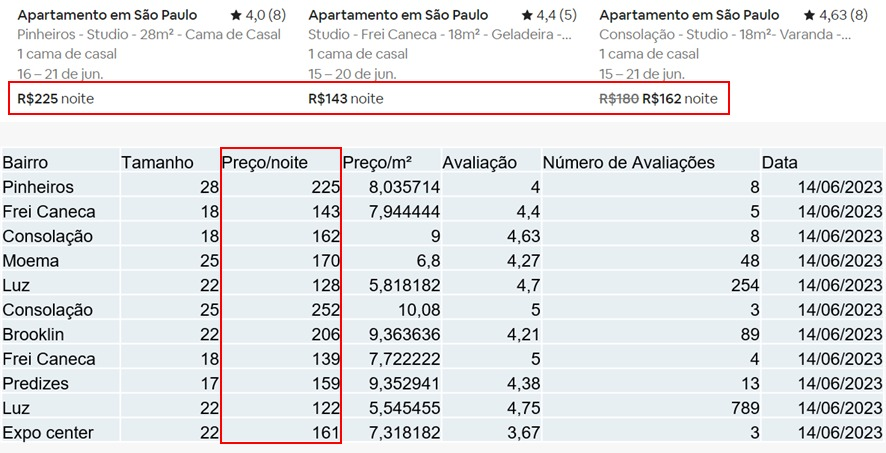
\includegraphics[width = .9\linewidth]{relatorios/lounge/imagens/img.jpg}

\bigskip

Para a plataforma do Air DNA foi preciso nos aprofundar mais ao 
utilizar das ferramentas do site, pois ele é bastante denso e tem diversas 
funções que poderiam nos ajudar na obtenção dos dados. Após explorar e 
discutir em grupo, decidiu-se criar algo com informações mais regionais e 
visuais dentro da cidade de São Paulo, justamente para complementar as 
informações vindas das extrações do Air BNB, veja exemplos dos resultados.

\begin{figure}
    \begin{subfigure}{0.49\linewidth}
        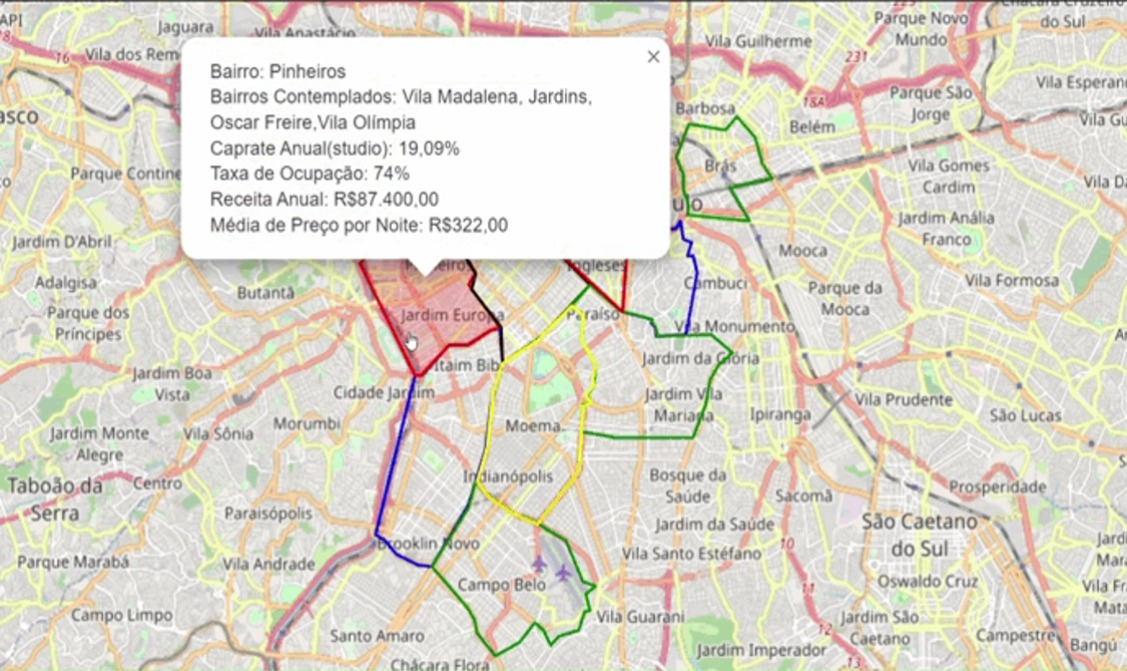
\includegraphics[width = \textwidth]{relatorios/lounge/imagens/1.jpg}
    \end{subfigure}
    \hfill
    \begin{subfigure}{0.49\linewidth}
        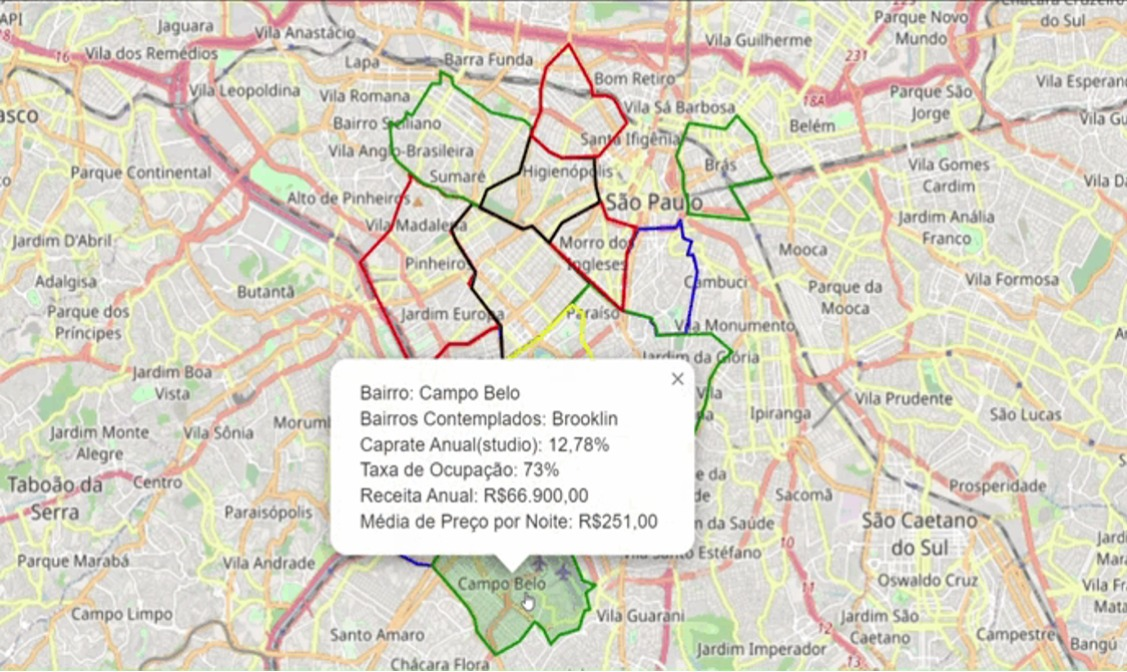
\includegraphics[width = \textwidth]{relatorios/lounge/imagens/2.jpg}
    \end{subfigure}
    \begin{subfigure}{0.49\linewidth}
        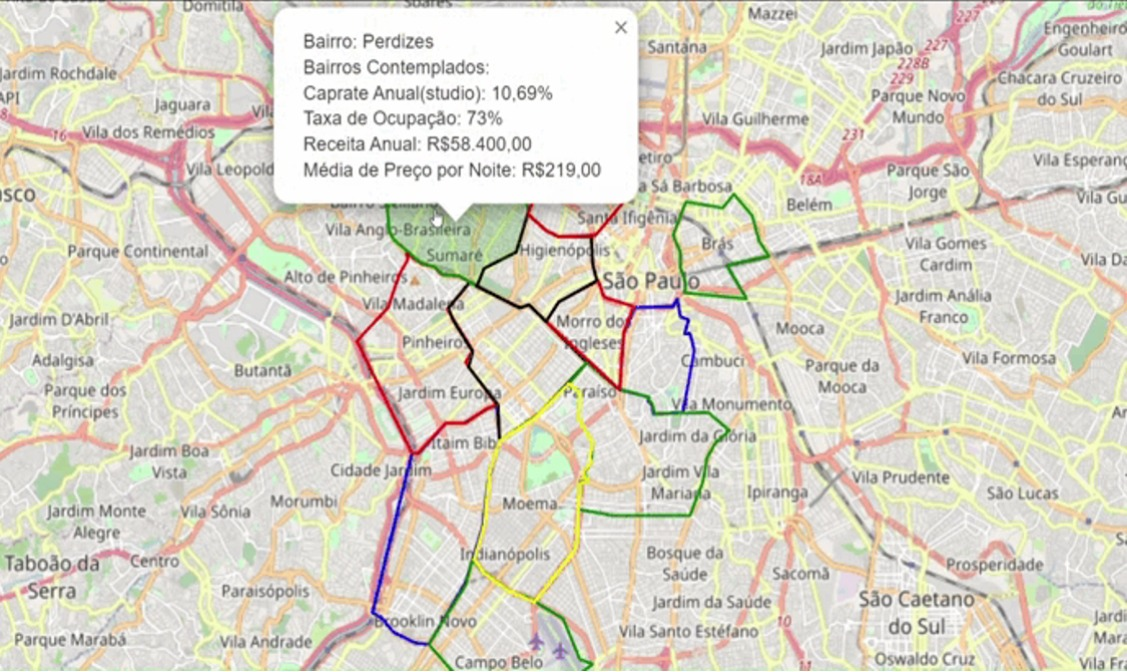
\includegraphics[width = \textwidth]{relatorios/lounge/imagens/3.jpg}
    \end{subfigure}
    \hfill
    \begin{subfigure}{0.49\linewidth}
        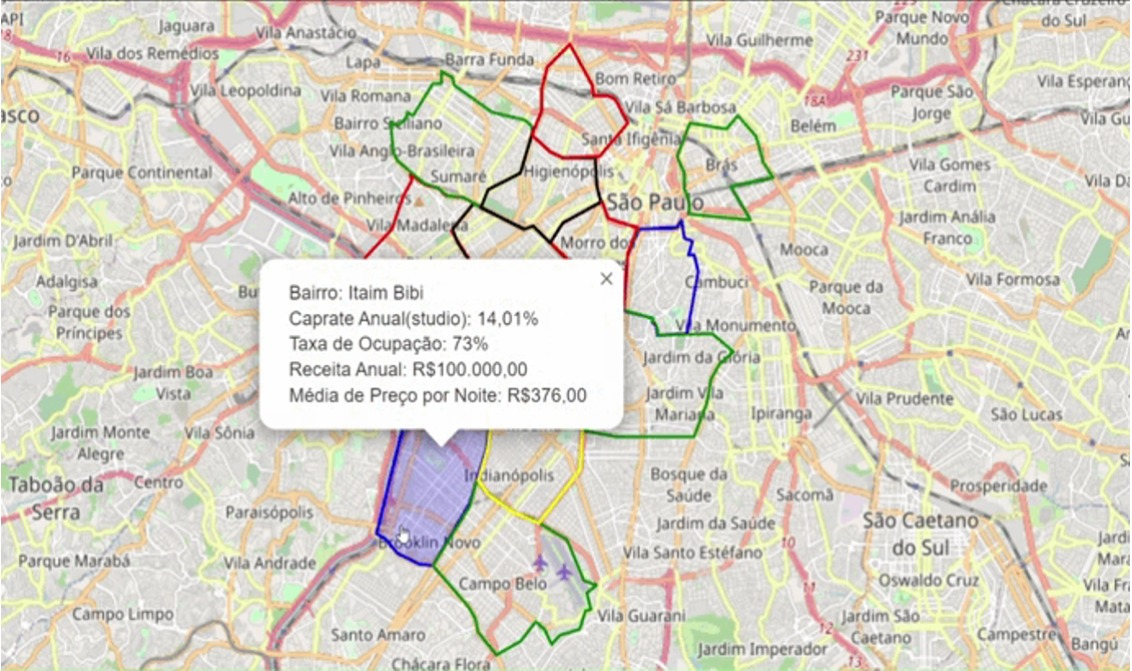
\includegraphics[width = \textwidth]{relatorios/lounge/imagens/4.jpg}
    \end{subfigure}

\end{figure}



\section*{Desafios}

As mudanças de planos em si foi uma dificuldade para nós, afinal quando
ocorreu, o rumo do projeto era completamente diferente e, com o tempo 
passando, a cobrança por resultados começou a ficar mais pesada.

A metodologia para a extração de dados foi u desafiadora também, afinal, 
apesar da biblioteca utilizada ter sido a mesma, os códigos foram bem diferentes, 
pois o Air DNA funciona por assinatura, diferente do Air BNB.

Entretanto, ao longo do semestre, o grupo conseguiu se adaptar bem ao que 
foi proposto e superou as dificuldades, em geral os resultados obtidos foram 
satisfatórios e agora cabe a Lounge 161 utilizar as ferramentas fornecidas pelo 
Insper Data para realizar uma modelagem eficiente tendo em vista o tema central 
do projeto.

\section*{Agradecimentos}

Dentro do Insper Data, recebemos diversas ajudas para desenvolver nosso 
projeto, porém, de forma especial gostaríamos de agradecer ao Presidente Thiago Rocha 
e o Diretor de Projetos André Correa, eles nos deram bons direcionamentos em 
momentos chaves do projeto.

Gostaríamos de agradecer também à Lounge 161 pela confiança depositar em 
nossos esforços para agregar em seus serviços profissionais, de modo especial, Enzo 
Pravatta e Leonardo Franuci que acompanharam o projeto dede o início e mantiveram 
contado e ciência em nossos avanços e desenvolvimentos